\documentclass[a4paper]{article}
\usepackage[utf8]{inputenc}
\usepackage[spanish, es-tabla]{babel}

\usepackage[a4paper, footnotesep = 1cm, width=18cm, left=2cm, top=2.5cm, height=25cm, textwidth=18cm, textheight=25cm]{geometry}
%\geometry{showframe}

\usepackage{amsmath}
\usepackage{amsfonts}
\usepackage{amssymb}
\usepackage{float}
\usepackage{graphicx}
\usepackage{caption}
\usepackage{subcaption}
\usepackage{multicol}
\usepackage{multirow}
\setlength{\doublerulesep}{\arrayrulewidth}

\usepackage{hyperref}
\hypersetup{
    colorlinks=true,
    linkcolor=blue,
    filecolor=magenta,      
    urlcolor=blue,
    citecolor=blue,    
}

\newcommand{\quotes}[1]{``#1''}
\usepackage{array}
\newcolumntype{C}[1]{>{\centering\let\newline\\\arraybackslash\hspace{0pt}}m{#1}}
\usepackage[american]{circuitikz}
\usepackage{fancyhdr}
\usepackage{units} 

\pagestyle{fancy}
\fancyhf{}
\lhead{22.11 Electrónica I}
\rhead{Mechoulam, Lambertucci, Rodriguez, Londero}
\rfoot{Página \thepage}

\begin{document}

%%%%%%%%%%%%%%%%%%%%%%%%%
%		Caratula		%
%%%%%%%%%%%%%%%%%%%%%%%%%

\begin{titlepage}
\newcommand{\HRule}{\rule{\linewidth}{0.5mm}}
\center
\mbox{\textsc{\LARGE \bfseries {Instituto Tecnológico de Buenos Aires}}}\\[1.5cm]
\textsc{\Large 22.11 Electrónica I}\\[0.5cm]


\HRule \\[0.6cm]
{ \Huge \bfseries Trabajo práctico N$^{\circ}$1}\\[0.4cm] 
\HRule \\[1.5cm]


{\large

\emph{Grupo 3}\\
\vspace{3px}

\begin{tabular}{lr} 	
\textsc{Mechoulam}, Alan  &  58438\\
\textsc{Lambertucci}, Guido Enrique  & 58009 \\
\textsc{Rodriguez Turco}, Martín Sebastian  & 56629 \\
\textsc{Londero Bonaparte}, Tomás Guillermo  & 58150 \\
\end{tabular}

\vspace{20px}

\emph{Profesores}\\
Alcocer, Fernando\\
Oreglia, Eduardo Victor\\
Gardella, Pablo Jesús\\
\vspace{3px}
%\textsc{} \\	

\vspace{100px}

\begin{tabular}{ll}

Presentado: & 24/09/19\\

\end{tabular}

}

\vfill

\end{titlepage}


%%%%%%%%%%%%%%%%%%%%%
%		Indice		%
%%%%%%%%%%%%%%%%%%%%%

\tableofcontents
\newpage

%%%%%%%%%%%%%%%%%%%%%
%		Informe		%
%%%%%%%%%%%%%%%%%%%%%
\section{Introducción}
En el siguiente informe se busca analizar, desarrollar y confeccionar algún circuito estudiado a lo largo del cuatrimestre. Se destaca la existencia de una dificultad adicional, la cual se basa en el método mediante el cual se fueron adquiriendo los componentes. Estos fueron subastados durante la cursada, entre los diversos grupos. De esta forma, se condiciona el circuito final, ya que se posee acceso limitado a estos, los cuales no se pudieron elegir libremente.

\section{Desarrollo}

\subsection{Componentes dispuestos}
El presente grupo se valió de los siguientes componentes:
\begin{itemize}
	\item Dos pares de resistencias de $6.8 \ k\Omega$ y de $680 \ k\Omega$.
	\item Un transistor BJT NPN. 
	\item Un diodo 1N4148.
	\item Un JFET.
	\item Un par Darlington NPN.
	\item Una placa de 5x5.
\end{itemize}

\subsection{Circuitos considerados}
Como primer opción se consideró utilizar el par Darlington y mediante el uso de las resistencias, configurarlo de forma tal que este quede compensado. Una alternativa es el uso de una fuente de corriente, con el mismo objetivo que se mencionó anteriormente.
\begin{figure}[H]
\centering
\begin{subfigure}{.45\textwidth}
\centering
	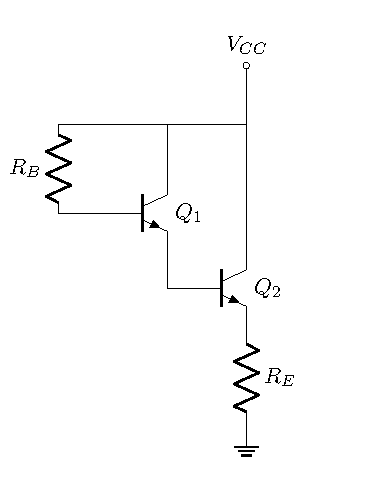
\includegraphics[width=0.5\textwidth, page=1]{Imagenes/ParDarlington.pdf}
	\caption{Par Darlington.}
	\label{fig:pardar1}
\end{subfigure}
\begin{subfigure}{.4\textwidth}
\centering
	\includegraphics[width=0.6\textwidth, page=2]{Imagenes/ParDarlington.pdf}
	\caption{Par Darlington compensado con $R$.}
	\label{fig:pardar2}
\end{subfigure}
\begin{subfigure}{.5\textwidth}
\centering
	\includegraphics[width=0.5\textwidth, page=3]{Imagenes/ParDarlington.pdf}
	\caption{Par Darlington compensado con fuente de corriente.}
	\label{fig:pardar3}
\end{subfigure}
\caption{Configuraciones y modificaciones posibles para el par Darlington.}
\label{fig:pardar}
\end{figure}

La conexión representada en la Figura (\ref{fig:pardar1}) no es conveniente. Una de las principales desventajas consiste en que si es deseable aumentar la ganancia de tensión del sistema, se debe modificar el valor de $R_E$, modificando también la polarización del sistema.

Por otro lado, la mostrada en la Figura (\ref{fig:pardar2}) permite aumentar la corriente $I_{CEQ1}$ y aprovecharla de cierta forma llevándola al colector de $Q_2$. Una variación mejor de esta configuración es colocar la resistencia a tierra, ya que de esta forma permite extraer más corriente de $Q_1$.

Finalmente, la mostrada en la Figura (\ref{fig:pardar3}) es la más optima para compensar el circuito, ya que permite polarizar el transistor $Q_2$ mediante corriente. Una particularidad de esta disposición es que la fuente empleada actúa tanto en la polarización como una carga activa. Además, de esta forma, es posible aumentar $I_{CEQ}$ sin modificar otros factores del propio circuito.

Cabe aclarar que, la disposición presentada en la Figura (\ref{fig:pardar2}), estrictamente hablando, es la más económica al problema anterior. Dadas las condiciones, dicha consideración no afecta en la decisión a implementar, ya que se cuenta con componentes para realizar cualquiera de las tres. También se destaca que se puede colocar un diodo entre el colector y el emisor de $Q_2$. Este tipo de configuración es utilizada para trabajar con potencias altas. Dado que este enfoque no es de interés, se reserva dicho componente.

\subsection{Fuente de corriente}
\label{subsec:fdei}
Una vez determinado que la implementación optima, con los componentes disponibles, es la presentada en la Figura~(\ref{fig:pardar3}), se decide confeccionarla. Para ello, primero se opta por analizar la fuente de corriente. Esta puede ser realizada con el JFET, dispuesto en una configuración en la cual se autopolarice, como se presenta a continuación.
\begin{figure}[H]
\centering
	\includegraphics[width=0.25\textwidth, page=4]{Imagenes/ParDarlington.pdf}
	\caption{Fuente de corriente.}
	\label{fig:fuentei}
\end{figure}

Recorriendo la malla de entrada y de salida del circuito de la Figura (\ref{fig:fuentei}), se obtienen las siguientes ecuaciones:
\begin{equation}
	V_{GS} = V_{SS} - I_{DS} R_{S}
\end{equation}
\begin{equation}
	V_{DS} = V_{DD} + V_{SS} - I_{DS} \left( R_{D} + R_{S} \right)
\end{equation}

Además, se plantean las ecuaciones del JFET:
\begin{equation}
\begin{split}
	I_{DS} = I_{DSS} & \left( 1 - \frac{V_{GS}}{V_P} \right)^2 \\
	gm = & \ 2\frac{\sqrt{I_{DS} I_{DSS}}}{|V_P|}
\end{split}
\end{equation}

De esta forma, seleccionando el componente \href{https://www.onsemi.com/pub/Collateral/2N3819-D.PDF}{2N3819}, se obtiene de la hoja de datos los valores de interés, tales como $I_{DSS} = 2 \ mA$ y $V_P = -8 \ V$ (para el peor caso). Luego, estableciendo $V_{SS} = 10 \ V$, $R_S = 6.8 \ K\Omega$ y $R_D = 680 \ \Omega$ se calculan la corriente de drain y la tensión gate-source. Como es de esperarse, se obtienen dos valores posibles para cada variable:
\begin{equation*}
\left\lbrace
\begin{split}
	&I_{DS} =  4.39 \ mA \\
	&V_{GS} =  -19.85 \ V
\end{split}
\right.
\ \ y \ \
\left\lbrace
\begin{split}
	&I_{DS} =  1.60 \ mA \\
	&V_{GS} =  -0.88 \ V
\end{split}
\right.
\end{equation*}

Sabiendo que se debe cumplir que $I_{DSS} \geq I_{DS}$ y $V_{GS} > V_{P}$, se descartan los primeros valores, seleccionando $I_{DS} = 1.60 \ mA$ y $V_{GS} = -0.88 \ V$, obteniéndose así $gm = 0.45 \ \frac{mA}{V}$. De esta forma se garantiza que esté polarizado adecuadamente. \textcolor{red}{Por otro lado, para garantizar que se cumpla $V_{DS} > V_{DSE} = |V_{GS} - V_P|$, se requiere el valor de $V_{DD}$. Dado que este circuito es empleado para polarizar otro, dicha tensión queda fijada por la totalidad del circuito, por lo que este análisis es expuesto más adelante.}

Con lo establecido previamente, se prosigue a plantear el circuito incremental. Es de interés calcular la impedancia de salida, para luego reemplazarla por su propia fuente en el análisis incremental del circuito de la Figura (\ref{fig:pardar3}).
\begin{figure}[H]
\centering
	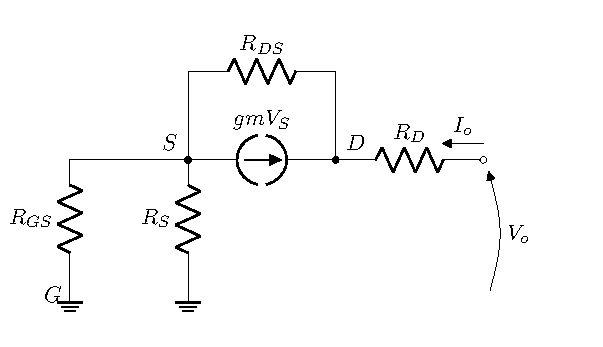
\includegraphics[width=0.45\textwidth, page=1]{Imagenes/ModeloIncremental.pdf}
	\caption{Circuito incremental de la Figura (\ref{fig:fuentei}).}
\label{fig:incfuente1}
\end{figure}

Se destaca que, como el gate queda a tierra, se cumple que $V_{GS} = V_G - V_S = - V_S$, por lo tanto, se da vuelta la fuente de corriente y se reemplaza con lo mencionado anteriormente. 

Se define $R_S^* = R_S // R_{GS}$, para luego analizar el circuito presentado en la Figura (\ref{fig:incfuente2}).
\begin{figure}[H]
\centering
\hspace*{2cm}
	\includegraphics[width=0.4\textwidth, page=2]{Imagenes/ModeloIncremental.pdf}
	\caption{Análisis de la impedancia de salida del circuito de la fuente de corriente.}
\label{fig:incfuente2}
\end{figure}

Planteando la tensión $V_o$ y las corrientes del nodo $D$, se obtienen las siguientes expresiones respectivamente.
\begin{equation*}
	V_o = I_{DS} R_{DS} + I_o \left( R_D + R_S^* \right)
\end{equation*}
\begin{equation*}
	I_{DS} = gm V_S + I_o = \left( gm R_S^* + 1 \right) I_o
\end{equation*}

Operando algebraicamente se obtiene la variable deseada de la forma:
\begin{equation}
\begin{split}
	R_{OF} & = \frac{V_o}{I_o} = R_{DS} \left( 1 + gm R_S^* \right) + R_S^* + R_D \\
		   & = R_{DS} \left( 1 + gm R_S//R_{GS} \right) + R_S//R_{GS} + R_D
\end{split}
\label{equ:rof}
\end{equation}

Para poder continuar, se toma $R_{GS} \longrightarrow \infty$, luego se asume $V_A = -90 \ V$, estimando así $R_{DS} = \frac{V_A}{I_{DS}} = 56.25 \ K\Omega$. De esta forma se obtiene de (\ref{equ:rof}) el valor de la impedancia de salida $R_{OF} \approx 234.79 \ K\Omega$.

\subsection{Darlington compensado por corriente}
Con lo obtenido en la Sección (\ref{subsec:fdei}), se posee la información necesaria para analizar el circuito presentado en la Figura (\ref{fig:pardar3}). En el análisis que se muestra a continuación se presentan la carga y la alimentación del sistema, componentes que no fueron presentados en la Figura (\ref{fig:pardar}) por cuestiones de simplicidad.
\begin{figure}[H]
\centering
	\includegraphics[width=0.5\textwidth, page=5]{Imagenes/ParDarlington.pdf}
	\caption{Circuito equivalente al reemplazar la fuente de corriente.}
	\label{fig:pardar4}
\end{figure}

A continuación, se seleccionan los transistores a utilizar en el par Darlington, eligiendo \href{https://www.sparkfun.com/datasheets/Components/BC546.pdf}{BC547} para este caso. Por un lado, como se está polarizando este transistor por corriente, se garantiza que $I_{CE2} = 1.60 \ mA$. Por otro lado, para el caso de $Q_1$, se plantea la malla de entrada, obteniéndose así la corriente $I_{CQ1}$ de la forma
\begin{equation*}
	V_{CC} - I_{B1} R_B - V_{BEON} - \left( I_{CQ1} - I_{B2} \right) R_E = 0
\end{equation*}
\begin{equation*}
	V_{CC} - V_{BEON} - I_{B2} R_E = I_{B1} R_B + I_{CQ1} R_E = I_{CQ1} \left( \frac{R_B}{h_{fe1}} + R_E \right)
\end{equation*}
\begin{equation}
	I_{CQ1} = \left( V_{CC} - V_{BEON} + I_{CQ2} \frac{R_E}{h_{FE2}} \right) \left( \frac{R_B}{h_{fe1}} + R_E \right)^{-1}
\end{equation}

Por otro lado, para la tensión $V_{CE1}$, se obtiene
\begin{equation}
	V_{CE1} = V_{CC} - I_{CQ1} R_E
\end{equation}

De esta forma, se tomando $V_{CC} = 12 \ V$, $R_E = 680 \ \Omega$ y $R_B = 6.8 \ k\Omega$, se obtiene $I_{CE1} = 15.25 \ mA$ y $V_{CE1} = 1.63 \ V$. Es así que, asumiendo $T = 27^o C$ y $V_{A1} = V_{A2} = V_A = -90 \ V$, y sabiendo que los estimadores empleados son $gm = \frac{I_{CE}}{V_T}$, $h_{ie} = \frac{h_{fe}}{gm}$ y $\frac{1}{h_{oe}} = \frac{V_A}{I_{CE}}$, se buscan conseguir los valores de los estimadores deseados. Para el caso de $h_{fe1}$ y $h_{hfe2}$ se observa de la hoja de datos el gráfico de $h_{ie}$ en función de la corriente del colector, presentada aquí en la Figura (\ref{fig:hfe-i}).
\begin{figure}[H]
\centering
	\includegraphics[width=0.4\textwidth, page=3]{Imagenes/Dc-Current-Gain.png}
	\caption{Ganancia de corriente continua.}
\label{fig:hfe-i}
\end{figure}

El hecho de que la corriente del colector del transistor $Q_2$ es aproximadamente 10 veces menor que la de $Q_1$ permite pensar que los $h_{fe}$ de cada transistor sean distintos, ya que ambas corrientes están separadas por una década de diferencia. En el caso presente, la situación es distinta, ya que para las corrientes obtenidas, se puede asumir que $h_{fe1} = h_{fe2} = 110$.

Luego, con todos los datos obtenidos y presentados, se elabora la siguiente tabla, en la cual se presentan los valores de los estimadores necesarios.
\begin{table}[H]
\centering
\begin{tabular}{cccc}
\hline
\textbf{Transistor} & $\mathbf{gm \ \left[ \frac{mA}{V} \right]}$ & $\mathbf{h_{ie} \ \left[ K\Omega \right]}$ & $\mathbf{\frac{1}{h_{oe} \ \left[ K\Omega \right]}}$ \\
\hline
$Q_1$ & 589.90 & 0.19 & 5.90 \\
$Q_2$ & 61.89 & 1.78 & 56.25	\\
\hline
\end{tabular}
\caption{Estimadores y datos pertinentes del modelo incremental del circuito Darlington.}
\label{tab:estim}
\end{table}

El siguiente paso consiste en reemplazar la fuente de corriente por su respectiva impedancia de salida $R_{OF}$. Planteando su respectivo modelo incremental, se llega al circuito presentado a continuación: 
\begin{figure}[H]
\centering
	\includegraphics[width=0.85\textwidth, page=3]{Imagenes/ModeloIncremental.pdf}
	\caption{Modelo incremental del par Darlington.}
\label{fig:incdar}
\end{figure}

Se observa en la Figura (\ref{fig:incdar}) que, se puede obtener una relación entre $I_{B2}$ y $I_o$, mediante el uso de un divisor de corriente, siendo esta
\begin{equation*}
	I_o = I_{B2} \left( 1 + h_{fe2} \right) \frac{R_{OF} // \frac{1}{h_{oe2}}}{R_L + R_{OF} // \frac{1}{h_{oe2}}}
\end{equation*}
\begin{equation}
	\frac{I_o}{I_{B2}} = \left( 1 + h_{fe2} \right) \frac{R_{OF} // \frac{1}{h_{oe2}}}{R_L + R_{OF} // \frac{1}{h_{oe2}}}
	\label{equ:io-ib2}
\end{equation}

Luego, definiéndose $R_{E}^* = R_{E} // \frac{1}{h_{oe1}}$ y $R_d = R_{OF} // \frac{1}{h_{oe2}} // R_L$, se obtiene
\begin{figure}[H]
\centering
	\includegraphics[width=0.8\textwidth, page=4]{Imagenes/ModeloIncremental.pdf}
\end{figure}

Aplicando paso a nivel de corriente para la fuente de $h_{ie2} I_{B2}$, se llega a
\begin{figure}[H]
\centering
	\includegraphics[width=0.8\textwidth, page=5]{Imagenes/ModeloIncremental.pdf}
\end{figure}

Por un lado se destaca que 
\begin{equation*}
	V_o = I_{B2} R_d \left( 1 + h_{fe2} \right)
\end{equation*}
\begin{equation}
	\frac{V_o}{I_{B2}} = R_d \left( 1 + h_{fe2} \right)
\label{equ:vo-ib2}
\end{equation}

Por otro lado, se puede hallar una relación entre $I_{B1}$ e $I_{B2}$, de la misma forma que se realizó con $I_o$ e $I_{B2}$, siendo así
\begin{equation*}
	I_{B2} = I_{B1} \left( 1 + h_{fe1} \right) \frac{R_{E}^*}{ R_{E}^* + h_{ie2} + R_d \left( 1 + h_{fe2} \right) }
\end{equation*}
\begin{equation}
	\frac{I_{B2}}{I_{B1}} = \left( 1 + h_{fe1} \right) \frac{R_{E}^*}{ R_{E}^* + h_{ie2} + R_d \left( 1 + h_{fe2} \right) }
	\label{equ:ib2-ib1}
\end{equation}

De manera análoga, se toma el equivalente al paralelo entre $R_{E}^*$ con $h_{ie2}$ y $R_d \left( 1 + h_{fe2} \right)$. Por lo tanto, se define $R_{d}^* = R_{E}^* // \left[ h_{ie2} + R_d \left( 1 + h_{fe2} \right) \right]$ para luego aplicar paso a nivel de corriente con la segunda fuente.
\begin{figure}[H]
\centering
	\includegraphics[width=0.6\textwidth, page=6]{Imagenes/ModeloIncremental.pdf}
\end{figure}

De esta forma, se observa que
\begin{equation*}
	V_i = I_{B1} \left[ h_{ie1} + R_{d}^* \left( 1 + h_{fe1} \right) \right]
\end{equation*}
\begin{equation}
	\frac{V_i}{I_{B1}} = h_{ie1} + R_{d}^* \left( 1 + h_{fe1} \right)
	\label{equ:vi-ib1}
\end{equation}

Finalmente, se planteando nuevamente un divisor de corrientes, se obtiene
\begin{equation*}
	I_{B1} = I_i \frac{R_B}{R_B + h_{ie1} + R_{d}^* \left(1 + h_{fe1} \right)}
\end{equation*}
\begin{equation}
	\frac{I_{B1}}{I_i} = \frac{R_B}{R_B + h_{ie1} + R_{d}^* \left(1 + h_{fe1} \right)}
	\label{equ:ib1-ii}
\end{equation}

Con lo obtenido en (\ref{equ:vo-ib2}), (\ref{equ:ib2-ib1}) y (\ref{equ:vi-ib1}), se procede a calcular la transferencia $\Delta V$, siendo esta de la forma
\begin{equation}
	\Delta V \triangleq \frac{V_o}{V_i} = \frac{V_o}{I_{B2}} \frac{I_{B2}}{I_{B1}} \frac{I_{B1}}{V_i} = \frac{ \left( 1+h_{fe2} \right) R_d}{h_{ie2}+ \left( 1+h_{fe2} \right) R_d} = 0.9897 \equiv -0.0897 \ dB
\label{equ:Av}
\end{equation}

Luego, se calcula la ganancia de corriente de manera similar. Utilizando (\ref{equ:io-ib2}), (\ref{equ:ib2-ib1}) y (\ref{equ:ib1-ii}), se obtiene
\begin{equation*}
	\Delta I \triangleq \frac{I_o}{I_i} = \frac{I_o}{I_{B2}} \frac{I_{B2}}{I_{B1}} \frac{I_{B1}}{I_i}
\end{equation*}
\begin{equation}
	\Delta I = \frac{R_C R_{E}^* R_B \left( 1 + h_{fe2} \right) \left( 1+h_{fe1} \right)}{ \left( R_{OF} R_L h_{oe2} + R_{OF} + R_L \right)  \left\lbrace \left[ \left( 1 + h_{fe2} \right) \left( 1 + h_{fe1} \right) R_d + h_{fe1} h_{ie2} + R_B + h_{ie2} \right] R_{E}^* + R_B \left[ h_{ie2} + \left( 1 + h_{fe2} \right) R_d \right]  \right\rbrace }
	\label{equ:Ai}
\end{equation}
\begin{equation*}
	\Delta I = 2.7673 \equiv 8.8412 \ dB
\end{equation*}

A continuación, se calcula la impedancia de entrada del amplificador, mediante el uso de (\ref{equ:vi-ib1}) y (\ref{equ:ib1-ii}), siendo esta
\begin{equation}
	R_{ia} = \frac{V_i}{I_i} =  \frac{V_i}{I_{B1}}\frac{I_{B1}}{I_i} = \frac{ R_B R_{E}^* \left[ h_{ie2} + \left( 1 + h_{fe2} \right) R_d \right] \left( 1 + h_{fe1} \right) }{ \left[ \left( 1 + h_{fe2} \right)  \left( 1 + h_{fe1} \right) R_d + h_{fe1} h_{ie2} + R_B + h_{ie2} \right] R_{E}^* + R_B \left[ h_{ie2} + \left( 1 + h_{fe2} \right) R_d \right] } = 6.1793 \ k\Omega
	\label{equ:Ria}
\end{equation}

Una vez obtenidos $\Delta V$ y $R_{ia}$, se puede calcular la ganancia de tensión del sistema $\Delta V_S$, siendo esta
\begin{equation}
\begin{split}
	\Delta V_S \triangleq \frac{V_S}{V_i} = \frac{V_S}{V_o} \frac{V_o}{V_i} = \frac{V_o}{V_i} \frac{R_{ia}}{R_S + R_{ia}} = 0.9075 \equiv -0.8432 \ dB
\end{split}
\label{equ:Avs}
\end{equation}

Por otro lado, para el calculo de la impedancia de salida $R_{oa}$ se considera el circuito de la siguiente forma:
\begin{figure}[H]
\centering
	\includegraphics[width=0.8\textwidth, page=7]{Imagenes/ModeloIncremental.pdf}
\end{figure}
Se definen $R_{S}^* = \left( R_B // R_S \right) + h_{ie1}$ y $R_{OF}^* = R_{OF} // \frac{1}{h_{oe1}}$. Luego, sabiendo que la tensión sobre $R_{E}^*$ y $R_{S}^*$ es la misma, se obtiene
\begin{equation}
	I_{OF} = I_{B1} \frac{R_{S}^*}{R_{E}^*}
	\label{equ:roa1}
\end{equation}

Luego, observando el nodo $E_2$, se llega a
\begin{equation}
	I_{B2} \left( 1 + h_{fe2} \right) + I_o = \frac{V_o}{R_{OF}^*}
	\label{equ:roa2}
\end{equation}

Se expresa la tensión $V_o$ como
\begin{equation}
	V_o = - \left( I_{B1} h_{ie1} + I_{B2} h_{ie2} \right)
	\label{equ:roa3}
\end{equation}
y se plantea para el nodo $C_1$, utilizando (\ref{equ:roa1}), llegándose a la expresión
\begin{equation}
	I_{B1} \left( 1 + h_{fe1} \right) + I_{OF} + I_{B2} h_{ie2} + I_o = \frac{V_o}{R_{OF}^*}
	\label{equ:roa4}
\end{equation}

De esta forma, con (\ref{equ:roa2}), (\ref{equ:roa3}) y (\ref{equ:roa4}), se opera algebraicamente y se obtiene finalmente la impedancia de salida del circuito
\begin{equation}
R_{oa} = \frac{V_o}{I_o} = 
\frac {R_{OF}^* \left[ \left( h_{fe1} + 1 \right) R_{E}^* + R_{S}^* \right] \left( 1 + h_{fe2} \right) }{ \left[ \left( h_{ie2} R_{OF}^* + 3 h_{fe2} + 3 \right) h_{fe1} + h_{ie2} R_{OF}^* + h_{fe2} + 1 \right] R_{E}^* + \left( h_{ie2} R_{OF}^* + h_{fe2} + 1 \right) R_{S}^* }
\end{equation}

\subsection{Desarrollo y armado de la placa}
\begin{center}
	\LARGE{\textcolor{red}{\textbf{Esquemático, PCB y foto.}}}\\
	\LARGE{\textcolor{red}{\textbf{Consideraciones necesarias para medir.}}}
\end{center}

\subsection{Mediciones}

\section{Conclusiones}
Dado que se optó por confeccionar una configuración Darlington, se puede afirmar que la ganancia de corriente del circuito, la cual ya de por sí es grande, como se demostró en \textcolor{red}{\textbf{(...)}}, es mayor que la de los demás grupos, ya que la principal característica de este es la alta ganancia de dicha variable. Por otro lado, también es posible afirmar que la polarización resulta altamente estable, ya que se logró efectuar la polarización mediante una fuente de corriente.
	
\end{document}